\chapter{Design}

\section{Overall System Design}

\subsection{Short description of the main parts of the system}
\textbf{Main Menu}\\
This will consist of a search bar button, an exit button, an add company button and a delete company button.\\
\textbf{Results Page}\\
This will consist of all of the relevant results to the item searched, the search bar in the top right of the window, an Edit information button, an Add information button and a Delete information button.\\
\textbf{Company Information Page}\\
This page will consist of all of the information about the specific company selected. It will show each of the suppliers phone number, owners name, email address, part provided, part price, address and website.\\
\textbf{Comments Section}\\
This page will consist of all the comments other employees have left. It will also have an "add comment" button that allows employees to add new comments.\\

\subsection{System flowcharts showing an overview of the complete system}
\begin{center}
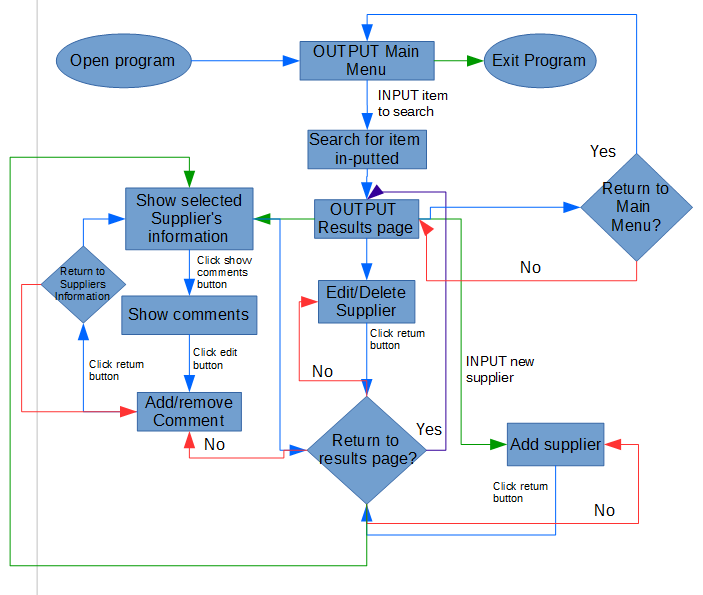
\includegraphics{Design Flowchart.png}
\end{center}
\section{User Interface Designs}

\section{Hardware Specification}

\section{Program Structure}

\subsection{Top-down design structure charts}

\subsection{Algorithms in pseudo-code for each data transformation process}

\subsection{Object Diagrams}

\subsection{Class Definitions}

\section{Prototyping}

\section{Definition of Data Requirements}

\subsection{Identification of all data input items}

\subsection{Identification of all data output items}

\subsection{Explanation of how data output items are generated}

\subsection{Data Dictionary}

\subsection{Identification of appropriate storage media}

\section{Database Design}

\subsection{Normalisation}

\subsubsection{ER Diagrams}

\subsubsection{Entity Descriptions}

\subsubsection{1NF to 3NF}

\subsection{SQL Queries}

\section{Security and Integrity of the System and Data}

\subsection{Security and Integrity of Data}

\subsection{System Security}

\section{Validation}

\section{Testing}

\begin{landscape}
\subsection{Outline Plan}

\begin{center}
    \begin{tabular}{|p{2cm}|p{5cm}|p{5cm}|p{4cm}|}
        \hline
        \textbf{Test Series} & \textbf{Purpose of Test Series} & \textbf{Testing Strategy} & \textbf{Strategy Rationale}\\ \hline
        Example & Example & Example & Example \\ \hline
    \end{tabular}
\end{center}

\subsection{Detailed Plan}

\begin{center}
    \begin{longtable}{|p{1.5cm}|p{2.5cm}|p{2.5cm}|p{2cm}|p{2cm}|p{2cm}|p{2cm}|p{2cm}|}
        \hline
        \textbf{Test Series} & \textbf{Purpose of Test} & \textbf{Test Description} & \textbf{Test Data} & \textbf{Test Data Type (Normal/ Erroneous/ Boundary)} & \textbf{Expected Result} & \textbf{Actual Result} & \textbf{Evidence}\\ \hline
        Example & Example & Example & Example & Example & Example & Example & Example \\ \hline
    \end{longtable}
\end{center}
\end{landscape}